%! Author = gabriel
%! Date = 5/7/23

% Preamble
\documentclass[12pt]{beamer}

% Packages
\usepackage{amsmath}
\usepackage{setup/packages}

\usetheme{Madrid}
\usecolortheme[named=darkgray]{structure}
\setbeamercolor{background canvas}{bg=gray}
%\setbeamercolor{frametitle}{bg=darkgray}
\setbeamercolor{footline}{bg=darkgray, fg=white}
\setbeamercolor{author in head/foot}{fg=white}
\setbeamertemplate{enumerate items}[default]
\setbeamertemplate{itemize item}[circle]
\setbeamertemplate{itemize subitem}[circle]
\setbeamertemplate{sections/subsections in toc}[sections numbered]
\setbeamercolor{section in toc}{fg=black}
\setbeamercolor{bibliography entry note}{fg=black, bg=white}
\setbeamertemplate{navigation symbols}{}
%\setbeamercolor{titlelike}{fg=white}
%\usefonttheme{structuresmallcapsserif}
\usefonttheme{serif}
%\setbeamertemplate{note page}[compress]
\setbeameroption{show notes on second screen}
\title{Problemas de Empacotamento}
\subtitle{métodos de solução baseados em \textit{bottom-left}}
\author[\href{https://github.com/G-Carneiro}{Gabriel Carneiro}]{
    \href{https://github.com/G-Carneiro}{Gabriel Medeiros Lopes Carneiro} \\
    Orientador: Pedro Belin Castellucci \\
    Coorientador: Rafael de Santiago
}
\institute[UFSC]{Universidade Federal de Santa Catarina}

\logo{\includegraphics[scale=0.05]{utils/images/vertical_sigla_PB_fundo_claro}}
\titlegraphic{
    \includegraphics[scale=0.15]{utils/images/vertical_sigla_PB_fundo_claro}
}
%
\setbeamertemplate{title page}[default][rounded=true]
%\setbeamertemplate{footline}{
%    \leavevmode%
%    \hbox{%
%        \begin{beamercolorbox}[wd=0.7\paperwidth,ht=2.25ex,dp=1ex,leftskip=1em]{footline}%
%            \includegraphics[scale=0.05]{utils/images/logo-ufsc}\hspace*{1em}%
%            \usebeamerfont{author in head/foot}\href{https://github.com/G-Carneiro}{Gabriel Carneiro}
%        \end{beamercolorbox}%
%%        \begin{beamercolorbox}[wd=.3\paperwidth,ht=2.25ex,dp=1ex,center]{title in head/foot}%
%%            \usebeamerfont{title in head/foot}\insertshorttitle
%%        \end{beamercolorbox}%
%        \begin{beamercolorbox}[wd=.3\paperwidth,ht=2.25ex,dp=1ex,right]{date in head/foot}%
%%            \usebeamerfont{date in head/foot}\insertshortdate{}\hspace*{2em}
%            \insertframenumber{} / \inserttotalframenumber\hspace*{2ex}
%        \end{beamercolorbox}}%
%    \vskip0pt%
%}

\addbibresource{aftertext/references.bib}

% Document
\begin{document}
    \begin{frame}[plain]
        \titlepage
        \note{
            Meu nome é Gabriel e hoje vou apresentar uma prévia do meu tcc.

            O trabalho trata sobre métodos de solução baseados em \textit{bottom-left} para
            problema de empacotamento, ele foi feito sob orientação do professor Pedro e teve
            coorientação do professor Rafael.
        }
    \end{frame}

    \begin{frame}
        \frametitle{Sumário}
        \tableofcontents[hideallsubsections]
        \note{
            Vou começar explicando alguns termos que devo usar ao longo da apresentação.

            Depois vou explicar o problema em si, passando por suas características e classificações.

            Vou mostrar o que é \textit{bottom-left}, como ela funciona e
            as adaptações feitas com base nela.

            Também vou mostrar os resultados obtidos ao rodar instâncias de teste.

            Por fim, vou apresentar algumas conclusões que podem ser feitas a partir do trabalho.
        }
    \end{frame}


    \section{Conceitos básicos}\label{sec:introducao}

\subsection{Modelos de otimização}\label{subsec:modelos-de-otimizacao}
\begin{frame}
    \frametitle{Modelos de otimização}
    \[
        \min\!/\!\max f(x), x \in \mathcal{X}.
    \]
    \begin{itemize}
        \item $x$: variável de decisão, $x = x_1, x_2, \dots, x_n$.
        \item $\mathcal{X}$: conjunto factível ou domínio;
        \item $f(x)$: função objetivo.
    \end{itemize}
    \note{
        Modelos de otimização são aproximações da realidade, representam o problema de
        maneira simples e objetiva, usando restrições.
        Geralmente quer minimizar ou maximizar uma função $f(x)$ com $x$
        obedecendo algumas restrições.
        \begin{itemize}
            \item $x$: variável de decisão, $x = x_1, x_2, \dots, x_n$.
            \item $\mathcal{X}$: conjunto factível ou domínio,
            possui todas as soluções possíveis para o problema.
            \item $f(x)$: função objetivo, a qual determinará o critério de escolha da solução.
        \end{itemize}
    }
\end{frame}

\subsection{Tipos de soluções}\label{subsec:tipos-de-solucoes}
\begin{frame}
    \frametitle{Tipos de soluções}
    \begin{itemize}
        \item Factível.
        \begin{itemize}
            \item Ótima.
            \item Problema ilimitado.
        \end{itemize}
        \item Problema infactível.
    \end{itemize}
    \note{
        \begin{itemize}
            \item Factível: satisfaz todas as restrições do problema.
            \item Ótima: melhor solução factível.
            \item Problema ilimitado: não é possível encontrar uma solução ótima,
            ou seja, sempre é possível achar uma melhor.
            \item Problema infactível: quando o problema não possui solução,
            geralmente devido a muitas restrições.
        \end{itemize}
    }
\end{frame}

\begin{frame}
    \frametitle{Conceitos básicos}
    \framesubtitle{Modelo contínuo $\times$ discreto}
    \begin{figure}[!htb]
        \centering
        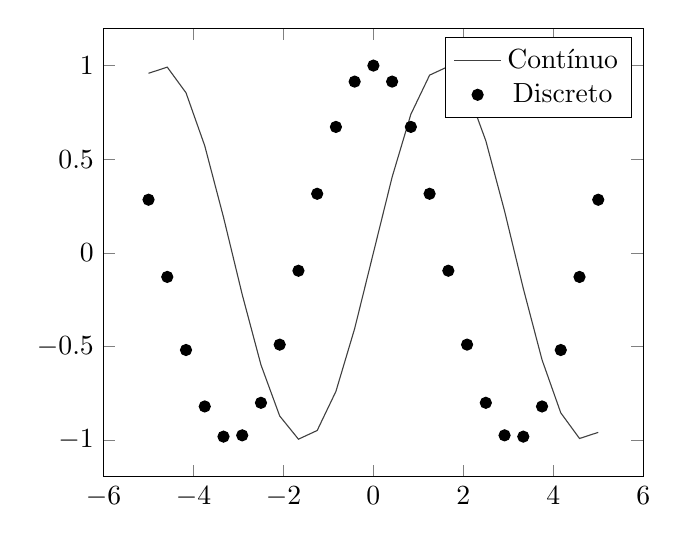
\begin{tikzpicture}
            \begin{axis}
                \addplot[darkgray] {sin((deg(x))};
                \addplot[black, only marks] {cos(deg(x))};
                \legend{Contínuo, Discreto};
            \end{axis}
        \end{tikzpicture}
        \caption{Exemplo de modelo contínuo e discreto.}
        \label{fig:continuo-discreto}
    \end{figure}
    \note{
    % TODO: explicar sobre domínios convexos não convexos
        Um modelo é contínuo quando sua região factível é contínua, ou seja, dado um ponto
        dessa região todos os seus vizinhos também serão uma solução.

        Modelos discretos não possuem seu domínio contínuo.
    }
\end{frame}

\subsection{Métodos exatos × heurísticos}\label{subsec:metodos-exatos-heuristicos}
\begin{frame}
    \frametitle{Métodos exatos × heurísticos}
    \begin{columns}
        \begin{column}{0.5\textwidth}
            Exatos
            \begin{itemize}
                \item Solução ótima.
                \item Tempo.
                \item Recursos.
            \end{itemize}
        \end{column}
        \begin{column}{0.5\textwidth}
            Heurísticos
            \begin{itemize}
                \item Solução factível.
                \item Simplicidade.
                \item Grande porte.
            \end{itemize}
        \end{column}
    \end{columns}
    \note{
        Métodos exatos sempre vão garantir a solução ótima para o problema,
        porém encontrar tal solução pode requerer grande tempo
        e/ou muitos recursos computacionais.

        Já heurísticas buscam por soluções factíveis
        e são geralmente usadas em problemas de grande porte.

        O problema de interesse é NP-difícil, então buscar uma solução ótima fica
        praticamente inviável devido a limitações de tempo e recursos computacionais.
        Uma heurística será utilizada para obter uma solução boa em tempo hábil.
    }
\end{frame}

    \section{Problema}\label{sec:problema}
\begin{frame}
    \frametitle{Problema}
    Alocar peças em um espaço.
    \begin{itemize}
        \item Difícil resolução.
        \item $N$-dimensional.
        \item Tipos de peças.
        \item Classificação.
        \item Variantes.
    \end{itemize}
    \note{
        A premissa do problema é simples, alocar peças em um espaço.
        Pode parecer algo bobo de resolver, mas é de difícil resolução já que pode possuir
        $N$-dimensões e diversos tipos de peças, de modo que é preciso separar o problema em
        diferentes classes e ainda existem variantes dentro das classificações.
    }
\end{frame}

\subsection{N-dimensões}\label{subsec:n-dimensoes}
\begin{frame}
    \frametitle{Problema}
    \framesubtitle{$N$-dimensões}
    \begin{figure}[!htb]
        \centering
        \caption{Represeção 1D, 2D e 3D.}
        \includegraphics[scale=0.6]{utils/images/packing-example}
        \caption*{Fonte: \citeauthoryear{castellucci2019consolidation}.}
        \label{fig:packing}
    \end{figure}
    \note{
        Como eu disse, o problema pode ter $N$-dimensões, aqui vou citar alguns exemplos.
        \begin{itemize}
            \item O caso 1D pode ser usado para empilhar caixas de mesma profundidade e largura.
            \item Já no 2D poderia ser aplicado em casos onde somente a profundidade é fixa.
            \item E o 3D seria alocar caixas em um depósito ou container.
            \item O trabalho se concentra somente no caso 2D.
        \end{itemize}
    }
\end{frame}

\subsection{Restrições}\label{subsec:restricoes}
\begin{frame}
    \frametitle{Problema}
    \framesubtitle{Restrições}
    \scriptsize{
        \begin{align}
            x_i \in \{0, \dots, W - w_i\}, y_i \in \{0, \dots, H - h_i\} \left(i \in \mathcal{I}'\right) \label{eq:1} \\
            [x_i, x_i + w_i) \cap [x_j, x_j + w_j) = \emptyset \text{ ou } [y_i, y_i + h_i) \cap [y_j, y_j + h_j) = \emptyset \left(i, j \in \mathcal{I}', i \neq j\right) \label{eq:2}
        \end{align}
    }
    \note{
        Como já definimos a dimensão do problema, podemos ver as restrições do modelo.

        A primeira restrição garante que um item só é alocado no recipiente se couber nele.

        Já a segunda impede sobreposição entre as peças.
    }
\end{frame}

    \section{\textit{Bottom-left}}\label{sec:bottom-left}
\begin{frame}
    \frametitle{\textit{Bottom-left}}
    \begin{figure}[!htb]
        \centering
        \includegraphics[scale=0.8]{utils/images/bottom-left}
        \caption{Representação de alocação.}
        \caption*{Fonte:\cite{aprendizado-reforco}}
        \label{fig:bottom-left}
    \end{figure}
    \note{
        Como o problema é NP-difícil uma heurística será usada e a \textit{bottom-left}
        foi a escolhida.

        Ela é bem simples, dado uma lista como entrada, os itens são retirados um a um
        e posicionados no ponto mais a baixo a mais a esquerda quanto for possível.

        Caso a peça não caiba em nenhuma posição ela não entra na solução e passa-se para
        a próxima da fila.

        Aqui fica claro que a sequência de alocação tem impacto direto na qualidade da solução.
        Então como definir essa ordenação? Existe algum critério que se sobressai dos demais?
    }
\end{frame}

\subsection{Critérios de ordenação}\label{subsec:criterios-de-ordenacao}
\begin{frame}
    \frametitle{Critérios de ordenação}
    \begin{itemize}
        \item Área.
        \item Perímetro.
        \item Largura.
        \item Altura.
        \item Id.
    \end{itemize}
    \note{
        5 critérios de ordenação foram escolhidos: área, perímetro, largura, altura e id.

        A ordenação por id considera a ordem em que os itens foram colocados na lista (ou criados),
        ou seja, seria a forma padrão de resolver.

        Cada critério pode ser usado de forma crescente ou decrescente.
    }
\end{frame}

\subsection{Regiões}\label{subsec:regioes}
\begin{frame}
    \frametitle{Regiões}
    \begin{itemize}
        \item Vertical.
        \item Horizontal.
        \item $\max$(área).
        \item Nenhuma.
    \end{itemize}
    \note{
        As regiões são criadas de 4 formas diferentes, traçando uma linha vertical,
        uma horizontal, traçando uma linha (vertical ou horizontal) que maximize a área de uma das
        regiões geradas e com nenhuma linha.

        Nesse último modo sobreposições de peças podem ocorrer, então verificações
        são necessárias para cumprir a restrição.
    }
\end{frame}

\subsection{Testes}\label{subsec:testes}
\begin{frame}
    \frametitle{Testes}
    \begin{itemize}
        \item 45 instâncias.
        \begin{itemize}
            \item BKW\@.
            \item GCUT\@.
            \item NGCUT\@.
            \item OF\@.
            \item OKP\@.
        \end{itemize}
        \item 5 testes por configuração.
        \item $45 \cdot 5 \cdot 2 \cdot 4 \cdot 5 = 9000$ execuções.
        \item ±5 horas.
    \end{itemize}
    \note{
        Para testar os métodos de solução criados foram usados 5 conjuntos de instâncias:
        BKW, GCUT, NGCUT, OF e OKP, totalizando 45 instâncias de teste.

        Cada método foi executado 5 vezes em cada uma das instâncias para se obter um média,
        também foi calculado a mediana e desvio padrão.

        Como temos 45 instâncias, 5 critérios de ordenação, cada critério pode ser crescente ou
        decrescente, 4 formas de criar regiões e cada uma dessas combinações foi executada 5
        vezes, temos o total de 9000 execuções.

        O tempo somado de todas as execuções foi de aproximadamente 5 horas (valor que ainda
        será alterado, pois falta rodar a maior instância com o método de solução mais demorado).
    }
\end{frame}
    \section{Resultados}\label{sec:resultados}

\subsection{Testes}\label{subsec:testes}
\begin{frame}
    \frametitle{Resultados}
    \framesubtitle{Testes}
    \begin{itemize}
        \item 45 instâncias.
        \item $45 \cdot 5 \cdot 2 \cdot 4 = 1800$ casos de teste.
        \item 5 testes por configuração.
        \item $1800\cdot 5 = 9000$ execuções.
    \end{itemize}
    \note{
        Para testar os métodos de solução criados foram usadas 45 instâncias de teste.

        Como temos 45 instâncias, 5 critérios de ordenação, cada critério pode ser crescente ou
        decrescente, e 4 formas de criar regiões, temos o total de 1800 casos a serem testados.

        Cada método foi executado 5 vezes em cada uma das instâncias para se obter um média,
        totalizando 9000 execuções.
    }
\end{frame}

\subsection{Comparativo - Ordenação}\label{subsec:configuracoes-ruins}
\begin{frame}
    \frametitle{Resultados}
    \framesubtitle{Ordenação}

    \only<1>{
        \begin{table}
            \centering
            \caption{Comparativo entre ordenação crescente e decrescente.}
            \label{tab:descending}
            \small\ttfamily\begin{tabular}{lrrrr}
    \hline
    Decrescente & Vitórias & Empates & Qualidade \% & Tempo (s)  \\
    \hline
    Sim         & 736      & 8       & 78.9136      & 1.7798e+00 \\
    Não         & 167      & 8       & 57.3060      & 2.3715e+00 \\
    \hline
\end{tabular}
        \end{table}
    }
    \only<2>{\begin{figure}[H]
    \centering
    \includegraphics[scale=0.5]{output/figures/bkw/bkw01/horizontally/height/false/00}
    \caption{Regiões criadas na ordenação crescente - estado inicial.}
    \label{fig:estado-inicial}
\end{figure}
}
    \only<3>{\begin{figure}[H]
    \centering
    \caption{Regiões criadas na ordenação crescente - estado 1.}
    \includegraphics[scale=0.5]{output/figures/bkw/bkw01/horizontally/height/false/01}
    \label{fig:estado-1}
    \fonte{feito pelo autor.}
\end{figure}
}
    \only<4>{\begin{figure}
    \centering
    \includegraphics[scale=0.5]{output/figures/bkw/bkw01/horizontally/height/false/02}
    \caption{Regiões criadas na ordenação crescente - estado 2.}
    \label{fig:estado-2}
\end{figure}
}
    \only<5>{\begin{figure}
    \centering
    \includegraphics[scale=0.5]{output/figures/bkw/bkw01/horizontally/height/false/06}
    \caption{Regiões criadas na ordenação crescente - estado final.}
    \label{fig:estado-final}
\end{figure}
}
    \note<1>{
        Nas tabelas, a coluna “Qualidade” indica qualidade da solução obtida pelo método, ou seja,
        a porcentagem, em média, da área ocupada dos recipientes.
        A coluna “Vitórias” indica quantas vezes o critério obteve o melhor resultado e a coluna
        “Empates” indica quantas vezes obteve o melhor resultado, mas não foi o único a conseguir.
        A primeira coisa que fica evidente com os resultados é discrepância
        na qualidade de solução entre a ordenação crescente e a decrescente, algo já esperado.}
    \note<2>{Isso se deve a como as regiões são criadas, as figuras mostram o caso para
    ordenação crescente pela altura e linha horizontal para criação de regiões.}
    \note<3>{Ao posicionar uma peça uma das regiões ficará com a mesma altura do item
    recém-posicionado, como a ordenação é crescente a próxima peça terá no mínimo
    a mesma altura, mas o provável é que seja mais alta, impossibilitando que seja
    alocada nessa região.}
    \note<4>{O mesmo ocorre para o segundo e demais itens, fazendo com que muitas regiões fiquem
    sem poder receber peças.}
    \note<5>{Essa figura mostra o estado final do algoritmo e grande parte do espaço
    ainda está livre, mas não será preenchido. Algo semelhante ocorre com outros critérios de
    ordenação e criação regiões.}
\end{frame}

\begin{frame}
    \frametitle{Resultados}
    \framesubtitle{Critérios de ordenação}
    \begin{table}
        \centering
        \caption{Resultado para os critérios de ordenção.}
        \label{tab:order}
        \small\ttfamily\begin{tabular}{lrrrr}
    \hline
    Ordenação & Vitórias & Empates & Qualidade \% & Tempo (s)  \\
    \hline
    Área      & 63       & 39      & 82.7353      & 1.5874e+00 \\
    Perímetro & 71       & 38      & 84.6986      & 1.5769e+00 \\
    Altura    & 40       & 16      & 77.4182      & 1.5655e+00 \\
    Largura   & 66       & 24      & 81.1899      & 2.0805e+00 \\
    Id        & 16       & 5       & 68.5261      & 2.0889e+00 \\
    \hline
\end{tabular}
    \end{table}
    \note{
        Em relação aos critérios de ordenação, fica claro que ter algum critério de ordenação
        melhora e muito a solução, já que ordernar por ID teve um péssimo desempenho.
        Mas o curioso é que todos os demais critérios são competitivos entre si.
        A literatura em geral usa somente ordenação pela área~\cite{chen2019efficient}, esses
        resultados podem indicar que algumas instâncias possuem características que torne mais
        interessante outro método de ordenação.}
\end{frame}

\begin{frame}
    \frametitle{Resultados}
    \framesubtitle{Regiões}
    \begin{table}
        \centering
        \caption{Comparativo entre criação de regiões.}
        \label{tab:regioes}
        \small\ttfamily\begin{tabular}{lrrrrr}
\hline
Região & Wons & Draws & Quality \% & Items \% & Time (s)   \\
\hline
V      & 98   & 79    & 76.4030    & 45.0191  & 2.7157e-03 \\
H      & 70   & 60    & 75.9970    & 45.5439  & 6.2101e-03 \\
M      & 104  & 89    & 79.7175    & 47.6795  & 1.3743e-02 \\
N      & 176  & 119   & 83.6420    & 47.2335  & 7.2176e+00 \\
\hline
\end{tabular}
    \end{table}
    \note{Indo para o comparativo entre regiões percebemos que a que permite sobreposições se saiu
    melhor, tanto em quantitativa quanto qualitativa, ainda que na maioria dos casos não foi a única
    que encontrou a melhor solução, porém com um custo altíssimo de tempo.
    Regiões criadas com linhas verticais e horizontais foram mais rápidas, mas com soluções de pior
    qualidade. Enquanto maximizando as regiões levou um pouco a mais de tempo, mas também
    com acréscimo na qualidade. Aqui a gente percebe que ter sobreposição demora em torno de
    1000 vezes mais.}
\end{frame}

\begin{frame}
    \frametitle{Resultados}
    \framesubtitle{Sobreposição}
    \begin{table}
        \centering
        \caption{Resultados para sobreposição.}
        \label{tab:sobreposicao}
        \small\ttfamily\begin{tabular}{lrrr}
    \hline
    Superposition & Quality \% & Time (s)   \\
    \hline
    No            & 90.8278    & 1.6299e+01 \\
    Yes           & 87.2957    & 2.8313e+02
    \hline
\end{tabular}
    \end{table}
    \note{Na última tabela eu trouxe os números da comparação entre regiões simples e complexas.
    Na primeira linha temos os resultados de todas as combinações possíveis com regiões simples
    e o tempo total que levou para executar todas as instâncias. Já na segunda linha somente a
    ordenação decrescente pela área e regiões complexas foi considerada, já que obteve os melhores
    resultados.
    Os demais critérios não foram considerados pois esse sozinho já ultrapassa o tempo de todos os
    métodos sem sobreposição, caso fossem considerados o tempo total seria cerca de 10 vezes maior
    enquanto a qualidade teria pouco acréscimo.
    Aqui fica nítido que compensa muito mais, tanto em qualidade quanto em tempo, rodar todas
    as combinações possíveis com regiões simples e escolher o melhor resultado.
    Mas por que tanta diferença no tempo de execução entre com e sem sobreposição?}
\end{frame}

\begin{frame}
    \frametitle{Resultados}
    \framesubtitle{Complexidade}
    \begin{itemize}
        \item Sem sobreposição: $R = O\left(\dfrac{n^2 + n}{2}\right)$.
        \item Com sobreposição: $\displaystyle R = O\left(\dfrac{n^2 + n}{2}\right),
        S = O\left(\dfrac{n^3 - n}{3}\right)$.
        $n = 3152 \to R = \numprint{4969128}, S = \numprint{10438481552}.$
        % $S = O\left(\sum_{i=1}^{n} i(i - 1)\right)$
        % https://brilliant.org/wiki/sum-of-n-n2-or-n3/
    \end{itemize}
    \note{Isso se deve a complexidade dos algoritmos.
    Como dito antes, sem sobreposições temos que checar se um item cabe em uma região, no pior
    caso teremos que fazer isso para $(n^2 + n) / 2$ regiões, onde $n$ é número de itens.
    Enquanto com sobreposição, além de ter esse número de regiões, para cada uma delas
    também é necessário checar possíveis sobreposições com as peças já alocadas, sendo o número
    de verificações igual a $(n^3 - n)/3$, isso no pior caso, algo custoso.
    Por exemplo, para uma instância com 3152 itens podem ser necessárias mais de 10 bilhões
    de verificações de sobreposição.
    Então, aquela diferença de 1000 vezes fica ainda maior de acordo com a quantidade de itens
    a serem alocados.}
\end{frame}


    \section{Conclusão}\label{sec:conclusao}
    \begin{frame}
        \frametitle{Conclusão}
        \begin{itemize}
            \item Múltiplos métodos de solução.
            \item Resultados inesperados.
            \item Com sobreposição $\times$ sem sobreposição.
        \end{itemize}
        \note{Bom, indo para as conclusões. Foram testados vários métodos de solução, todos
        baseados em \textit{bottom-left}, ficou evidente que ordenar a lista de entrada de forma
        decrescente é vantajoso.

        Tivemos alguns resultados inesperados como a competitividade entre todos os critérios de
        ordenação, sendo necessária uma investigação sobre características das instâncias. E também
        a pouca vantagem em termos de qualidade quando usamos regiões que permitem sobreposições.

        De modo geral, pode-se resolver um problema com todas as combinações que usem regiões sem
        sobreposição e buscar a de melhor solução, já que seu tempo de execução é pequeno.
        Resolver usando regiões com sobreposição só é recomendado em casos onde o modelo será usado
        mais de uma vez e sem alterações.}
    \end{frame}

    \begin{frame}[allowframebreaks]
        \frametitle{Referências}
        \framesubtitle{}
        \printbibliography\nocite{*}
        \note{}
    \end{frame}
\end{document}